L'architecture de Robozzle repose sur un principe de composition modulaire ascendante, inspiré des paradigmes de la programmation fonctionnelle. Chaque composant est construit à partir des éléments définis précédemment, formant une hiérarchie de concepts de complexité croissante.

\begin{figure}[h]
    \centering
    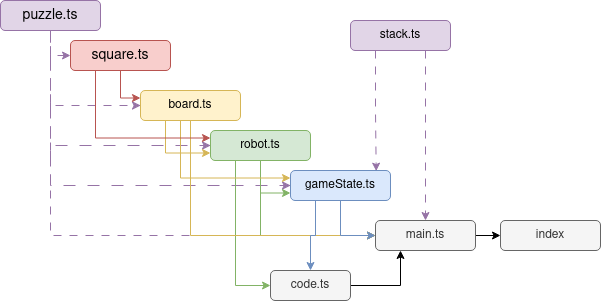
\includegraphics[width=0.6\textwidth]{archi_robot.png}
    \caption{Architecture du projet Robozzle}
    \label{fig:archi}
\end{figure}

Comme illustré par la figure \ref{fig:archi}, l’architecture repose à sa base sur le modules \textit{puzzle.ts}, qui contient des définitions de types et d’énumérations structurant le reste du code, et \textit{stack.ts}, chargé de l’implémentation de la pile.

Nous définissons le type de base \textit{Square} dans \textit{square.ts} représentant la cellule élémentaire de la grille de jeu. \`A partir de ce type , nous définissons le type abstrait \textit{Board}, un assemblage de squares de manière à former la grille de jeu, et puis \textit{Robot} qui est composé d’une position (définit par \textit{Square}) et une direction pour représenter un agent qui manipule un board.

Dans \textit{gameState.ts}, à partir de \textit{Board}, \textit{Robot} et \textit{Stack}, nous définissons l’état de jeu \textit{State}, capable de décrire de manière indépendante un jeu et son avancement, et une \textit{Action} qui modifie un \textit{State} en un autre faisant ainsi avancer la partie.

Finalement, avec les états de jeu, nous pouvons définir une interface de jeu via une couche graphique.

Cette approche reflète un principe fondamental de la programmation fonctionnelle : construire des abstractions complexes par composition de types simples sans recourir aux l'état mutable. Chaque module est autonome, testable isolément, et ne dépend que des couches inférieures. 
\\

Pour chaque couche, nous utilisons les types définis dans les couches inférieures comme briques de construction. \textit{Board} est construit à partir de \textit{Square}, \textit{Robot} à partir de \textit{Square} et \textit{Dir}, \textit{State} à partir de \textit{Board}, \textit{Robot} et \textit{Stack}. Chaque nouveau type abstrait enrichit les précédents sans les modifier, en les composant pour former une abstraction de niveau supérieur. C'est ce principe de composition ascendante qui donne à l'architecture sa cohérence : on ne repart jamais de zéro, on s'appuie sur ce qui est déjà défini et testé.

Nous remarquons dans la figure \ref{fig:archi} que plus les modules sont dans les couches externes au sens de dépendances et plus il dépendent d'un plus gros nombre de couches internes. Cela est visible principalement aux modules d'entrée au programme comme \textit{code.t} ou \textit{main.ts} qui doivent gérer tous ces modules.
